\documentclass[tikz,border=8pt]{standalone}
\usepackage{amsmath,amssymb}
\usetikzlibrary{arrows.meta,automata,positioning,quotes}
\begin{document}
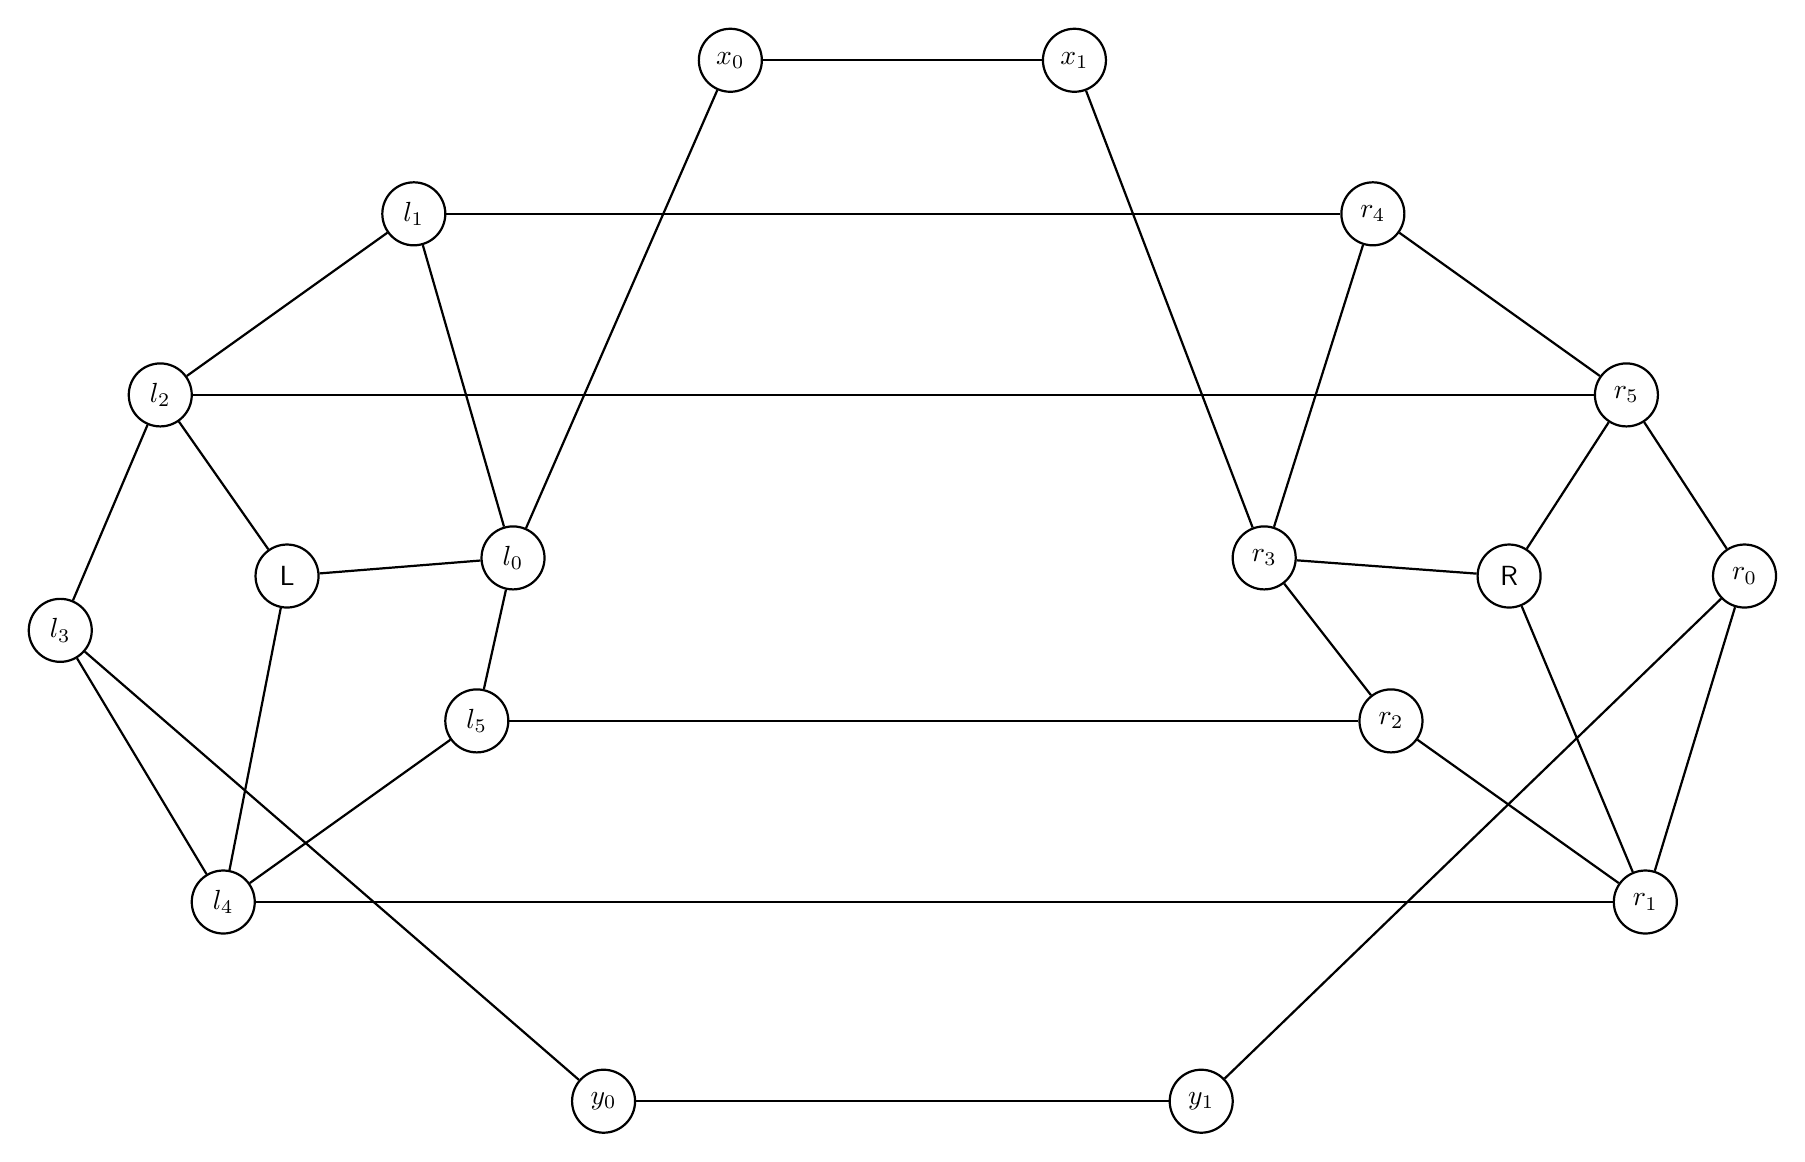
\begin{tikzpicture}[x=1cm,y=1cm]
\tikzset{
  graphnode/.style={circle,draw,thick,minimum size=8mm,inner sep=1pt,font=\sffamily},
  directed/.style={-{Stealth[length=2.4mm]},thick},
  undirected/.style={thick}
}
\node[graphnode] (n_L) at (-7.72,-0.21) {L};
\node[graphnode] (n_l0) at (-4.85,0.02) {$l_{0}$};
\node[graphnode] (n_l1) at (-6.11,4.39) {$l_{1}$};
\node[graphnode] (n_l2) at (-9.33,2.09) {$l_{2}$};
\node[graphnode] (n_l3) at (-10.60,-0.90) {$l_{3}$};
\node[graphnode] (n_l4) at (-8.53,-4.35) {$l_{4}$};
\node[graphnode] (n_l5) at (-5.31,-2.05) {$l_{5}$};
\node[graphnode] (n_R) at (7.80,-0.21) {R};
\node[graphnode] (n_r0) at (10.79,-0.21) {$r_{0}$};
\node[graphnode] (n_r1) at (9.53,-4.35) {$r_{1}$};
\node[graphnode] (n_r2) at (6.30,-2.05) {$r_{2}$};
\node[graphnode] (n_r3) at (4.69,0.02) {$r_{3}$};
\node[graphnode] (n_r4) at (6.07,4.39) {$r_{4}$};
\node[graphnode] (n_r5) at (9.29,2.09) {$r_{5}$};
\node[graphnode] (n_x0) at (-2.09,6.34) {$x_{0}$};
\node[graphnode] (n_x1) at (2.28,6.34) {$x_{1}$};
\node[graphnode] (n_y0) at (-3.70,-6.88) {$y_{0}$};
\node[graphnode] (n_y1) at (3.89,-6.88) {$y_{1}$};
\draw[undirected] (n_l0) -- (n_l1);
\draw[undirected] (n_l1) -- (n_l2);
\draw[undirected] (n_l2) -- (n_l3);
\draw[undirected] (n_l3) -- (n_l4);
\draw[undirected] (n_l4) -- (n_l5);
\draw[undirected] (n_l5) -- (n_l0);
\draw[undirected] (n_L) -- (n_l0);
\draw[undirected] (n_L) -- (n_l2);
\draw[undirected] (n_L) -- (n_l4);
\draw[undirected] (n_r0) -- (n_r1);
\draw[undirected] (n_r1) -- (n_r2);
\draw[undirected] (n_r2) -- (n_r3);
\draw[undirected] (n_r3) -- (n_r4);
\draw[undirected] (n_r4) -- (n_r5);
\draw[undirected] (n_r5) -- (n_r0);
\draw[undirected] (n_R) -- (n_r1);
\draw[undirected] (n_R) -- (n_r3);
\draw[undirected] (n_R) -- (n_r5);
\draw[undirected] (n_l0) -- (n_x0);
\draw[undirected] (n_x0) -- (n_x1);
\draw[undirected] (n_x1) -- (n_r3);
\draw[undirected] (n_l3) -- (n_y0);
\draw[undirected] (n_y0) -- (n_y1);
\draw[undirected] (n_y1) -- (n_r0);
\draw[undirected] (n_l1) -- (n_r4);
\draw[undirected] (n_l2) -- (n_r5);
\draw[undirected] (n_l4) -- (n_r1);
\draw[undirected] (n_l5) -- (n_r2);
\end{tikzpicture}
\end{document}
